\documentclass[a4page]{exam}
\usepackage{geometry}
\usepackage[table]{xcolor}
\usepackage{amsmath, amsfonts}
\usepackage{hyperref}
\usepackage{tikz}

\newcommand{\Str}[1]{\mathtt{#1}}

\title{Homework 3}
\author{CS 212 Nature of Computation\\Habib University\\Fall 2021}
\date{Due: 2359h on Sunday, 14 November}

\printanswers

\begin{document}
\maketitle
\thispagestyle{empty}

\noindent\rule{\textwidth}{1pt}

\begin{questions}
\question[20] Show that $\{a^i\#a^j \mid \frac{j}{k} = i \text{ for some positive integer } k\}$ is not context free, providing adequate reasoning for each class of cases of $uvxyz$ .

  \begin{solution}
    \textcolor{blue}{Solution by WS}.\\
    \textit{The key to this solution is to find the right $s$ that leads to a contradiction. The one used below exploits the fact that the maximum length that can be pumped at a time is $p$. The used $s$ is therefore long. For shorter strings, it becomes difficult to obtain contradictions. Also see }\href{https://math.stackexchange.com/questions/1971391/prove-that-f-ai-bj-mid-i-kj-text-for-some-positive-integer-k#comment4048973_1971397}{\textit{here.}}
    
    We can express the language as $L = \{a^i\#a^{ki} \mid k \in \mathbb{Z}^+\}$.

    We will prove that $L$ is not context-free through contradiction. Assume that $L$ is context-free. Then the pumping lemma holds. That is, there exists a length $p$ such that all strings, $s$, in $L$ with $|s| \geq p$ can be written as $s = uvxyz$ with substrings $u$, $v$, $x$, $y$, and $z$ such that
    \begin{enumerate}
    \item $|vy| > 0$,
    \item $|vxy| \leq p$, and
    \item $uv^ixy^iz \in L$ for all $i\geq 0$.
    \end{enumerate}

    Let us consider a string $s = a^{p+1}\#a^{(p+1)^2}$ where $p$ is the pumping length. We can see that $s\in L$ and that because $|s|\geq p$, the pumping lemma must apply to it. That is, $s$ can be broken down into substrings $u$, $v$, $x$, $y$, and $z$ which satisfy the above conditions. We do not know what these substrings are but we can reason about them based on the above conditions.
    
    From condition 1, we know that $v$ and $y$ are not both empty. Condition 3 states that \textit{pumping} $v$ and $y$ in $s$ by an equal amount yields strings in $L$. We can consider cases of $v$ and $y$.
    \begin{description}
    \item[Case 1. $v$ or $y$ contains \#:] Pumping up will yield multiple \#'s and the resulting string will not be in $L$. This is a contradiction. Alternately, we can say that this case cannot hold.
    \item[Case 2. $v$ or $y$ does not contain \#:] That is, they only contain $a$'s. This includes the case where either of them is $\epsilon$. We can consider three sub-cases depending on where $v$ and $y$ lie in $s$ with respect of the \#.
      \begin{description}
      \item[Case 2.1.  $v$ and $y$ on the left of \#:] Pumping up will eventually yield more $a$'s on the left of \# than on the right, and the resulting string will not be in $L$. This is a contradiction. Alternately, we can say that this case cannot hold.
      \item[Case 2.2. $v$ and $y$ on the right of \#:] Pumping down will reduce at most $p$ number of $a$'s on the right of \#. The resulting number of $a$'s on the right will no longer be a multiple of $(p+1)$ which is the number of $a$'s on the left of \#. Therefore the resulting string will not be in $L$. This is a contradiction. Alternately, we can say that this case cannot hold.
      \item[Case 2.3. $v$ on the left and $y$ on the right of \#:] Pumping up an arbitrary number of times will break the relationship between the number of $a$'s on the left and the right. Therefore the resulting string will not be in $L$. This is a contradiction. Alternately, we can say that this case cannot hold.
      \end{description}
    \end{description}

    We see that all cases lead to a contradiction. Or that no possible case can hold. Therefore, $L$ is not context-free.
  \end{solution}
  
\question[20] Show that every infinite Turing-recognizable language has an infinite Turing-decidable subset.
  \begin{solution}
    \textcolor{blue}{Solution taken from the submission by team \textit{class}}.\\
    In order to proof the given statement i.e. "every infinite Turing-recognizable language has an infinite Turing-decidable subset", we will assume an infinite turing recognizable language and an enumerator corresponding to that language. Then we will see that if for the said language and enumerator there exists any subset of infinite turing decidable language or not, which should be both infinite and turing decidable.
    
    So, Let $L$ be a turing recognizable language and $M$ be an enumerator that enumerates $L$. This is because we know that "a language is turing recognizable if and only if some enumerator enumerates it" (thoerm 3.2.1 in Introduction to theory of Computation - Micheal Sipser),
    
    Now consider a language $A = \{w_1,w_2,w_3,......, w_i\}$ where $w_1$ is the first string enumerated by $M$ and with increasing $i$ the string $w_{i-1}$ is smaller than $w_i$ lexicographically (alphabet wise).
    
    Using these assumptions, our goal is to proof two things listed below with their proofs.
    \begin{enumerate}
    \item $A$ is infinite and is a subset of $L$\\
      We can proof this using "proof by contradiction" method. Let us assume that $A$ is a finite language. The last string i.e $w_i$ is the largest string in $A$ lexicographically and all other strings enumerated by $M$ are lesser than ${w_i}$. Since there can be finite number of strings that are lesser than $w_i$, we say that $L$ (contains all string enumerated by $M$) would be finite. This is the contradiction because it is given that $L$ is infinite, it means that $A$ is also infinite. Hence proved that $A$ is infinite and is a subset of turing recognizable language $L$.    
      
    \item Next we have to prove that $A$ is decidable language. \\
      We know that a language is turing decidable if and only if some enumerator enumerates it in lexicographic order. Considering this, we can construct an enumerator $M'$ that must enumerate the language in lexicographic order. Such enumerator will perform following steps, 
      \begin{enumerate}
      \item Simulate $M'$ until it emits the string $t$. 
      \item if $t > w_i$ then replace $w_i$ with $t$.
      \item else ignore $t$.
      \item Resume simulating $M$ and go to step b. 
      \end{enumerate}
      As we are able to construct an enumerator that enumerated $A$ in lexicographic order, we say that $A$ is decidable.
    \end{enumerate}
    From both step 1 and step 2 we have proven that $A$ is an infinite decidable subset of $L$.
  \end{solution}
  
\question[20] Show that the class of Turing-recognizable languages is closed under concatenation.
  \begin{solution}
    \textcolor{blue}{Solution adapted from the submission by team \textit{complexity}}.\\
    Assume Turing machines $T_1$ and $T_2$ that recognize languages $L_1$ and $L_2$ respectively. Now, let's construct another non-deterministic TM, $T_3$ that recognizes language $L_1 L_2$ on input $w$.
    \begin{enumerate}
    \item Cut $w$ into $w_1$ and $w_2$ non-deterministically. 
    \item Considering every pair $(w_1, w_2)$, run $T_1$ on $w_1$. If it accepts, move to the next step, if it halts and rejects, reject. 
    \item Run $T_2$ on $w_2$, if it accepts, accept. If it halts and rejects, reject.
    \end{enumerate}
  \end{solution}

\question[20] Design a Turing Machine to decide the language
  \[
    L =\{ w w^{\text{rev}} : w \in \{a,b\}^* \},
  \]

  Your machine must halt on all inputs. Assume that the tape is infinite in both directions, with all characters other than the input initially blank. Give \textbf{both} the high-level idea behind your TM as well as a state diagram drawn in the conventional way. 
  \begin{solution}
    \textcolor{blue}{Solution taken from the submission by team \textit{theorem}}.\\
    The Turing Machine $\mathbf{TM}$ works as follows: Input $w$,
    \begin{enumerate}
    \item If $\mathbf{TM}$ reads $X$ or $Y$ then move right.\\
      Else if $\mathbf{TM}$ reads $\sqcup$ then accept. \\
      Else move to step 2. 
    \item If $\mathbf{TM}$ reads $a$ then
      \begin{itemize}
      \item write $X$
      \item move right
      \end{itemize}
      Else if $\mathbf{TM}$ reads $b$ then 
      \begin{itemize}
      \item write $Y$
      \item move right
      \end{itemize}
    \item Move right until $\mathbf{TM}$ reads $\sqcup$ or $X$ or $Y$.
    \item If $\mathbf{TM}$ reads $\sqcup$ or $X$, or $Y$, move left until it reads $a$ or $b$.
    \item If $\mathbf{TM}$ reads $a$ then 
      \begin{itemize}
      \item write $X$
      \item move left
      \end{itemize}
      Else if $\mathbf{TM}$ reads $b$ then 
      \begin{itemize}
      \item write $Y$
      \item move left
      \end{itemize}
    \item Move left until $\mathbf{TM}$ reads $X$ or $Y$.
    \item If $\mathbf{TM}$ reads $X$, or $Y$, move right and go to step 1
    \end{enumerate}
    
    Following is the state diagram of $\mathbf{TM}$. 

    \begin{center}
      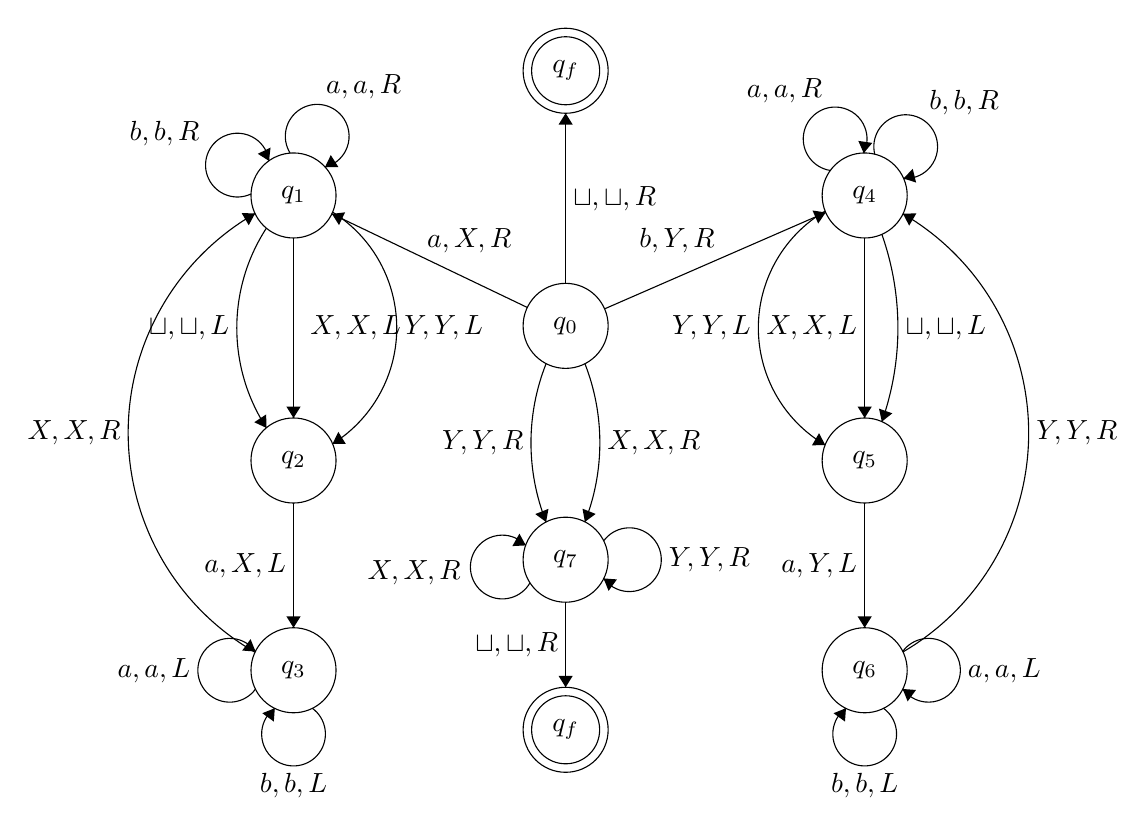
\begin{tikzpicture}[scale=0.18]
        \tikzstyle{every node}+=[inner sep=0pt]
        \draw [black] (37.9,-23.3) circle (3);
        \draw (37.9,-23.3) node {$q_0$};
        \draw [black] (18.7,-14.1) circle (3);
        \draw (18.7,-14.1) node {$q_1$};
        \draw [black] (18.7,-32.8) circle (3);
        \draw (18.7,-32.8) node {$q_2$};
        \draw [black] (18.7,-47.6) circle (3);
        \draw (18.7,-47.6) node {$q_3$};
        \draw [black] (59,-14.1) circle (3);
        \draw (59,-14.1) node {$q_4$};
        \draw [black] (59,-32.8) circle (3);
        \draw (59,-32.8) node {$q_5$};
        \draw [black] (59,-47.6) circle (3);
        \draw (59,-47.6) node {$q_6$};
        \draw [black] (37.9,-39.8) circle (3);
        \draw (37.9,-39.8) node {$q_7$};
        \draw [black] (37.9,-51.8) circle (3);
        \draw (37.9,-51.8) node {$q_{f}$};
        \draw [black] (37.9,-51.8) circle (2.4);
        \draw [black] (37.9,-5.3) circle (3);
        \draw (37.9,-5.3) node {$q_{f}$};
        \draw [black] (37.9,-5.3) circle (2.4);
        \draw [black] (35.19,-22) -- (21.41,-15.4);
        \fill [black] (21.41,-15.4) -- (21.91,-16.19) -- (22.34,-15.29);
        \draw (31.1,-18.18) node [above] {$a,X,R$};
        \draw [black] (18.468,-11.121) arc (212.18738:-75.81262:2.25);
        \draw (23.65,-7.29) node [above] {$a,a,R$};
        \fill [black] (20.92,-12.1) -- (21.87,-12.1) -- (21.33,-11.25);
        \draw [black] (15.714,-13.987) arc (295.5708:7.5708:2.25);
        \draw (12.09,-9.71) node [left] {$b,b,R$};
        \fill [black] (16.97,-11.66) -- (17.08,-10.72) -- (16.18,-11.16);
        \draw [black] (16.788,-30.497) arc (-146.9565:-213.0435:12.923);
        \fill [black] (16.79,-30.5) -- (16.77,-29.55) -- (15.93,-30.1);
        \draw (14.2,-23.45) node [left] {$\sqcup,\sqcup,L$};
        \draw [black] (18.7,-17.1) -- (18.7,-29.8);
        \fill [black] (18.7,-29.8) -- (19.2,-29) -- (18.2,-29);
        \draw (19.2,-23.45) node [right] {$\mbox{ }X,X,L$};
        \draw [black] (21.449,-15.272) arc (57.99615:-57.99615:9.644);
        \fill [black] (21.45,-31.63) -- (22.39,-31.63) -- (21.86,-30.78);
        \draw (26.48,-23.45) node [right] {$Y,Y,L$};
        \draw [black] (18.7,-35.8) -- (18.7,-44.6);
        \fill [black] (18.7,-44.6) -- (19.2,-43.8) -- (18.2,-43.8);
        \draw (18.2,-40.2) node [left] {$a,X,L$};
        \draw [black] (16.02,-48.923) arc (-36:-324:2.25);
        \draw (11.45,-47.6) node [left] {$a,a,L$};
        \fill [black] (16.02,-46.28) -- (15.67,-45.4) -- (15.08,-46.21);
        \draw [black] (20.023,-50.28) arc (54:-234:2.25);
        \draw (18.7,-54.85) node [below] {$b,b,L$};
        \fill [black] (17.38,-50.28) -- (16.5,-50.63) -- (17.31,-51.22);
        \draw [black] (15.987,-46.329) arc (-119.9194:-240.0806:17.859);
        \fill [black] (15.99,-15.37) -- (15.04,-15.34) -- (15.54,-16.2);
        \draw (6.54,-30.85) node [left] {$X,X,R$};
        \draw [black] (40.65,-22.1) -- (56.25,-15.3);
        \fill [black] (56.25,-15.3) -- (55.32,-15.16) -- (55.72,-16.08);
        \draw (45.76,-18.17) node [above] {$b,Y,R$};
        \draw [black] (56.587,-12.337) arc (261.58325:-26.41675:2.25);
        \draw (53.34,-7.61) node [above] {$a,a,R$};
        \fill [black] (58.93,-11.11) -- (59.54,-10.39) -- (58.55,-10.25);
        \draw [black] (59.712,-11.198) arc (193.95027:-94.04973:2.25);
        \draw (66.02,-8.44) node [above] {$b,b,R$};
        \fill [black] (61.74,-12.9) -- (62.63,-13.19) -- (62.39,-12.22);
        \draw [black] (60.211,-16.842) arc (19.49217:-19.49217:19.805);
        \fill [black] (60.21,-30.06) -- (60.95,-29.47) -- (60.01,-29.14);
        \draw (61.85,-23.45) node [right] {$\sqcup,\sqcup,L$};
        \draw [black] (59,-17.1) -- (59,-29.8);
        \fill [black] (59,-29.8) -- (59.5,-29) -- (58.5,-29);
        \draw (58.5,-23.45) node [left] {$X,X,L$};
        \draw [black] (56.22,-31.705) arc (-120.46867:-239.53133:9.578);
        \fill [black] (56.22,-31.71) -- (55.78,-30.87) -- (55.28,-31.73);
        \draw (51,-23.45) node [left] {$Y,Y,L$};
        \draw [black] (59,-35.8) -- (59,-44.6);
        \fill [black] (59,-44.6) -- (59.5,-43.8) -- (58.5,-43.8);
        \draw (58.5,-40.2) node [left] {$a,Y,L$};
        \draw [black] (61.68,-46.277) arc (144:-144:2.25);
        \draw (66.25,-47.6) node [right] {$a,a,L$};
        \fill [black] (61.68,-48.92) -- (62.03,-49.8) -- (62.62,-48.99);
        \draw [black] (60.323,-50.28) arc (54:-234:2.25);
        \draw (59,-54.85) node [below] {$b,b,L$};
        \fill [black] (57.68,-50.28) -- (56.8,-50.63) -- (57.61,-51.22);
        \draw [black] (61.704,-15.392) arc (59.66464:-59.66464:17.91);
        \fill [black] (61.7,-15.39) -- (62.14,-16.23) -- (62.65,-15.36);
        \draw (71.07,-30.85) node [right] {$Y,Y,R$};
        \draw [black] (36.524,-37.14) arc (-158.328:-201.672:15.136);
        \fill [black] (36.52,-37.14) -- (36.69,-36.21) -- (35.76,-36.58);
        \draw (34.95,-31.55) node [left] {$Y,Y,R$};
        \draw [black] (39.26,-25.968) arc (21.39575:-21.39575:15.3);
        \fill [black] (39.26,-37.13) -- (40.02,-36.57) -- (39.09,-36.2);
        \draw (40.81,-31.55) node [right] {$X,X,R$};
        \draw [black] (35.39,-41.421) arc (-29.41806:-317.41806:2.25);
        \draw (30.53,-40.69) node [left] {$X,X,R$};
        \fill [black] (35.09,-38.79) -- (34.64,-37.96) -- (34.14,-38.84);
        \draw [black] (40.58,-38.477) arc (144:-144:2.25);
        \draw (45.15,-39.8) node [right] {$Y,Y,R$};
        \fill [black] (40.58,-41.12) -- (40.93,-42) -- (41.52,-41.19);
        \draw [black] (37.9,-42.8) -- (37.9,-48.8);
        \fill [black] (37.9,-48.8) -- (38.4,-48) -- (37.4,-48);
        \draw (37.4,-45.8) node [left] {$\sqcup,\sqcup,R$};
        \draw [black] (37.9,-20.3) -- (37.9,-8.3);
        \fill [black] (37.9,-8.3) -- (37.4,-9.1) -- (38.4,-9.1);
        \draw (38.4,-14.3) node [right] {$\sqcup,\sqcup,R$};
      \end{tikzpicture}
    \end{center}

  \end{solution}

\question[20] The \texttt{FINITE INPUT ACCEPTANCE PROBLEM} is defined as the problem of deciding whether a given non-deterministic Turing Machine $M$ accepts input $x$ in $\leq k$ steps of computation. Derive an explanation for \texttt{FINITE INPUT ACCEPTANCE PROBLEM} being time-bounded by $O(n^k)$, where $n=|x|$. You will have to assume that the alphabet size is determined on the fly, based on the input.
  \begin{solution}
    \textcolor{blue}{Solution taken from the submission by team \textit{prefix}}.\\
     Let us define a Deterministic Turing Machine, $M_a$ that would solve the FINITE INPUT ACCEPTANCE PROBLEM
     for a non-deterministic Turing Machine $M$.
     Such a machine would take in input the string $x$, and simulate the machine $M$ for k steps. 
     
     If $M$ is able to accept $x$
     within k steps, then $M_a$ would go into the accepting state, which would state yes as the answer to the problem otherwise 
     it would go into the reject state which would proclaim the answer to be no.
     
     However, as $M_a$ is a deterministic machine simulating a nondeterministic machine, it would have to simulate
     each branch at a time, as explained in Theorm 3.16 in chapter 3 of "Introduction to theory of computation - Michael Sipser".
     
     So the machine $M_a$ would be performing a breadth first search over all nodes of the computation tree formed by $M$  
     upto the height $k$. The time taken by the machine, $T$, would be equivalent to the number of nodes it traverses.


    \includegraphics[width=.5\textwidth]{computation_tree.png}


    Considering the worst case where:\\
    - The maximum number of branches, $b$, occur in each step\\
    - The turing Machine $M$ does not accept in $k$ steps\\
    - $|\Sigma | = |x|$, as it is determined on input\\

    We can calculate the maximum number of branches, $b$:
    $$ b = |\text{max} \left( \mathcal{P}(Q \times \Gamma \times \{L\times R\}) \right) | $$
    $$ b = |Q| \times |\Gamma| \times 2 $$
    $$ b = |Q| \times (|\Sigma| + c) \times 2 \hspace{1mm} $$
    where $c$ is some arbitary constant representing the fixed number of additional charachter besides of $\Sigma$ 
    $$ b = 2 |Q| \times (|x| + c)$$
    $$ b = 2 |Q| \times (n + c)$$

    Then the time time taken by the machine, $T$, would be:
    $$ T = b^k $$
    $$ T = (2 |Q| \times (n + c))^k$$

    $$ O(T) = O((2 |Q| \times (n + c))^k)$$
    $$ O(T) = O(( |Q| \times n)^k)$$

    Let $n > p$, where $p$ is the pumping length of $M$ then $|Q|$ would remain constant as $n \to \infty$,
    Thus:

    $$ O(T) = O(n^k)$$

    As the machine $M_a$ is time bounded by $O(n^k)$ so would be  the FINITE INPUT ACCEPTANCE PROBLEM.

    Q.E.D
  \end{solution}
  
\end{questions}

\noindent\rule{\textwidth}{1pt}
\end{document}

%%% Local Variables:
%%% mode: latex
%%% TeX-master: t
%%% End:
